\documentclass[thesis.tex]{subfile}

\chapter{Implementation}
\label{ch:implementation}

Having previously discussed the goal of time-tiling, i.e.~to improve cache reuse by exploiting data locality between time iterations, this chapter presents our implementation of time-tiling in Devito, with reference to the design choices made.
For the most part, the implementation follows naturally from the previous chapters, although great care was required for the details, particularly the correct propagation of loop bounds under the transformations.

\wip{Rewrite para}
As outlined in Section~\ref{sec:bg-time-tiling}, we implement time-tiling in two stages: skewing in the DSE (Section~\ref{sec:skewing}), and tiling in the DLE (Section~\ref{sec:time-tiling}).
Finally, we consider the implications on sparse loops, one of Devito's raisons d'\^etre.


\section{Skewing}
\label{sec:skewing}
A loop nest comprises several nested loops, each with its own loop variable.
We may assume the outermost loop holds the time variable without loss of generality.\footnote{Otherwise, ignore any outer loops.}
In our implementation, incremental loop variables are increased by a factor of time, and the index accesses of that variable are decreased by the same factor in the loop body (Figures~\ref{lst:skewing-simple} and~\ref{fig:skewed-loops-skewed-space}).
In this way, all accesses refer to the same data as before the transformation, ensuring its validity.

\begin{figure}[!ht]
\begin{lstlisting}
for (int t = t_s; t < t_e; t++)
  for (int x = x_s; x < x_e; x++)
    A[t][x] = A[t-1][x-1] + A[t-1][x+1];

for (int t = t_s; t < t_e; t++)
  for (int x = x_s + t; x < x_e + t; x++)
    A[t][(x-t)] = A[t-1][(x-t)-1] + A[t-1][(x-t)+1];
\end{lstlisting}
	\caption{The code transformation of skewing: an unskewed loop, and a skewed version of the same loop. Note that all index accesses still refer to the same values.}
	\label{lst:skewing-simple}
\end{figure}

\begin{figure}[!ht]
\centering
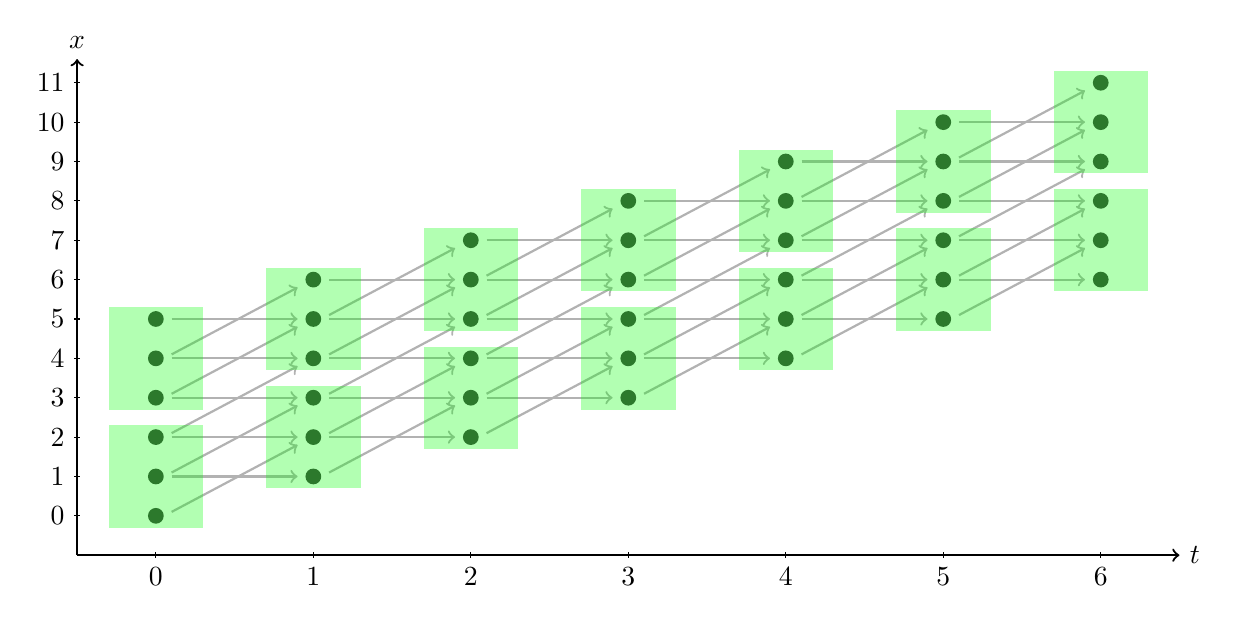
\begin{tikzpicture}
\draw[thick,->] (-1,-.5) -- (13,-.5) node[right]{$t$};
\draw[thick,->] (-1,-.5) -- (-1,5.8) node[above]{$x$};

\foreach \t in {0,1,2,3,4,5,6}
\foreach \x in {0,1,2,3,4,5}
\fill[darkgray] (\t*2,\x/2+\t/2) circle (0.1);

\foreach \t in {0,1,2,3,4,5}
\foreach \x in {1,2,3,4,5}
\draw[thick,->,gray!60] (\t*2+.2,\x/2+\t/2) -- (\t*2+1.8,\x/2+\t/2);

\foreach \t in {0,1,2,3,4,5}
\foreach \x in {0,1,2,3,4}
\draw[thick,->,gray!60] (\t*2+.2,\x/2+\t/2+.05) -- (\t*2+1.8,\x/2+\t/2+.9);

\foreach \t in {0,1,2,3,4,5,6}
\foreach \x in {0,3}
\fill[green,opacity=0.3] (\t*2-.6,\x/2+\t/2-.15) rectangle (\t*2+.6,\x/2+\t/2+1.15);

\foreach \t in {0,1,2,3,4,5,6}
\draw (\t*2,1pt-.5cm) -- (\t*2,-1pt-.5cm) node[anchor=north] {$\t$};
\foreach \x in {0,1,2,3,4,5,6,7,8,9,10,11}
\draw (1pt-1cm,\x/2) -- (-1pt-1cm,\x/2) node[anchor=east] {$\x$};
\end{tikzpicture}
\caption{A skewed iteration space. Dependencies between blocks have not changed, and interchange is \emph{not} valid. (Skewed) tiles included for reference.}
\label{fig:skewed-loops-skewed-space}
\end{figure}

Note that skewing \emph{does not} change the execution order of the loops, nor does it change the structure of the loop nest.

\subsection{Common sub-expression elimination}
\label{sec:impl-cse}

As skewing is merely a substitution of indices and loop bounds, we do not change the expressions.
Since arithmetic on floats is generally non-commutative, we especially wish to avoid changing the structure of expressions, to simplify testing of the code.

In particular, we ensure than skewing is performed \emph{before} CSE occurs, to avoid expansion during skewing.
CSE does not remove the skew, as it is partially applied in the loop header, and partially in the expression (see Figure~\ref{lst:skewing-simple}).

\subsection{Implementation}
This was a straightforward substitution in the Devito symbolic engine, exactly as described above.
We iterate over the dimensions, first identifying the time dimension, then adding the offset to each incremental spatial loop variable.
We then replace every reference to the space dimension variable with a similar reference, subtracting the offset.

If there is no time dimension, no skewing is applied, as time-tiling would not be relevant.


\section{Time-tiling}
\label{sec:time-tiling}
As we noted in the previous section, skewing has not changed the execution order: when applying the tiling transformation, we now have skewed tiles on a skewed iteration space (Figure~\ref{fig:skewed-loops-skewed-space}).
We now need to `straighten' the tiles by aligning the loop bounds.
All the transformations in this section pertain to tiling, and they are performed in the Devito loop engine.


\subsection{Aligning the loop bounds}
We need to modify the tiling transformation slightly to make the interchange valid.
This was explored in Section~\ref{sec:bg-time-tiling}.
As this alignment was achieved alongside bounding for valid array accesses (detailed in the next section), Figures~\ref{lst:skew-straight} and~\ref{fig:skew-straight} are for illustrative purposes only.

\begin{figure}[!ht]
\begin{lstlisting}
for (int t_blk = t_s; t_blk < t_e; t_blk += t_blk_size)
  for (int t = t_blk; t < min(t_e, t_blk + t_blk_size); t++)
    for (int x_blk = x_s; x_blk < x_e + t_e; x_blk += x_blk_size)
      for (int x = x_blk; x < min(x_e + t_e, x_blk + x_blk_size); x++)
        A[t][(x-t)] = A[t-1][(x-t)-1] + A[t-1][(x-t)+1];
\end{lstlisting}
	\caption{Code which has been tiled following a skewing transformation. This code contains invalid array accesses.}
	\label{lst:skew-straight}
\end{figure}

\begin{figure}[!ht]
	\centering
	\begin{tikzpicture}
	\draw[thick,->] (-1,-.5) -- (13,-.5) node[right]{$t$};
	\draw[thick,->] (-1,-.5) -- (-1,5.8) node[above]{$x$};
	
	\foreach \t in {0,1,2,3,4,5,6}
	\foreach \x in {0,1,2,3,4,5,6,7,8,9,10,11}
	\draw (\t*2,\x/2) node[cross=2.4,red]{};
	
	\foreach \t in {0,1,2,3,4,5,6}
	\foreach \x in {0,1,2,3,4,5}
	\fill[darkgray] (\t*2,\x/2+\t/2) circle (0.1);
	
	\foreach \t in {0,1,2,3,4,5}
	\foreach \x in {1,2,3,4,5}
	\draw[thick,->,darkgray!60] (\t*2+.2,\x/2+\t/2) -- (\t*2+1.8,\x/2+\t/2);
	
	\foreach \t in {0,1,2,3,4,5}
	\foreach \x in {0,1,2,3,4}
	\draw[thick,->,darkgray!60] (\t*2+.2,\x/2+\t/2+.05) -- (\t*2+1.8,\x/2+\t/2+.9);
	
	\foreach \t in {0,1,2,3,4,5,6}
	\foreach \x in {0,3,6,9}
	\fill[green,opacity=0.3] (\t*2-.6,\x/2-.15) rectangle (\t*2+.6,\x/2+1.15);
	
	\foreach \t in {0,1,2,3,4,5,6}
	\draw (\t*2,1pt-.5cm) -- (\t*2,-1pt-.5cm) node[anchor=north] {$\t$};
	\foreach \x in {0,1,2,3,4,5,6,7,8,9,10,11}
	\draw (1pt-1cm,\x/2) -- (-1pt-1cm,\x/2) node[anchor=east] {$\x$};
	\end{tikzpicture}
	\caption{Straightened tiles on a skewed iteration space. Invalid array accesses indicated by crosses.}
	\label{fig:skew-straight}
\end{figure}


\subsection{Min/max bounds for valid array accesses}
Since a skewed iteration space is not rectangular (or in general, not a hypercube), valid array accesses over a space variable will not be valid for the same values between time iterations (as seen the previous section).
As it is not feasible to generate a remainder loop for each time iteration and choice of space dimension,\footnote{This would require at least \(\sum_{m=1}^{n} \binom{n}{m} = 2^n \) remainder loop nests, where there are \(n\) spatial dimensions -- one for each choice of dimensions.} we bound the incremental loops using the \texttt{min} and \texttt{max} functions.

\begin{figure}[!ht]
\begin{lstlisting}
for (int t_blk = t_s; t_blk < t_e; t_blk += t_blk_size)
  for (int t = max(t_s, t_blk);
           t < min(t_e, t_blk + t_blk_size); t++)
    for (int x_blk = x_s; x_blk < x_e + t_e; x_blk += x_blk_size)
      for (int x = max(x_s + t, x_blk);
               x < min(x_e + t, x_blk + x_blk_size); x++)
        A[t][(x-t)] = A[t-1][(x-t)-1] + A[t-1][(x-t)+1];
\end{lstlisting}
	\caption{We add lower bounds for each of the incremental loop variables, and we change the upper bounds for the spatial dimensions to be bounded by \texttt{x\_e + t}, instead of \texttt{x\_e + t\_e}. This prevents out of bounds accesses in the lower and upper triangular regions of Figure~\ref{fig:skewing-bounded} respectively.}
	\label{lst:skewing-bounded}
\end{figure}

\begin{figure}[!ht]
\centering
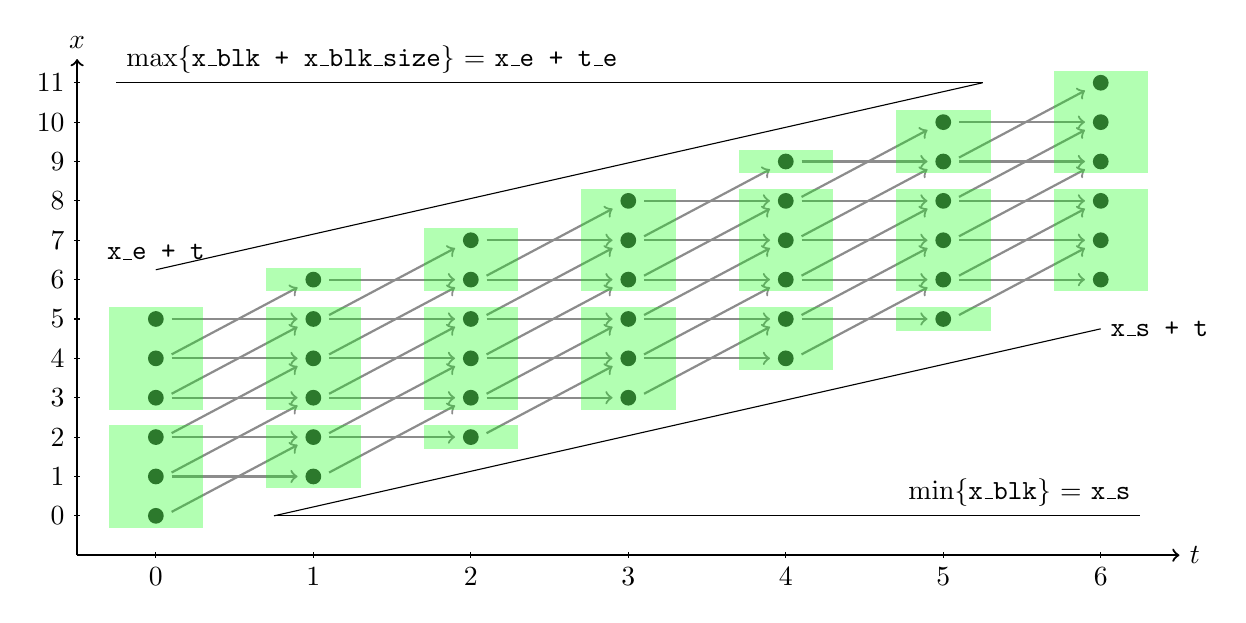
\begin{tikzpicture}
\draw[thick,->] (-1,-.5) -- (13,-.5) node[right]{$t$};
\draw[thick,->] (-1,-.5) -- (-1,5.8) node[above]{$x$};

% triangles
\draw (1.5,0) -- (12.5,0) node[anchor=south east] {min\{\texttt{x\_blk}\} = \texttt{x\_s}};
\draw (1.5,0) -- (12,2.375) node[anchor=west] {\texttt{x\_s + t}};
\draw (10.5,11/2) -- (-.5,11/2) node[anchor=south west] {max\{\texttt{x\_blk + x\_blk\_size}\} = \texttt{x\_e + t\_e}};
\draw (10.5,11/2) -- (0,3.125) node[anchor=south] {\texttt{x\_e + t}};

\foreach \t in {0,1,2,3,4,5,6}
\foreach \x in {0,1,2,3,4,5}
\fill[darkgray] (\t*2,\x/2+\t/2) circle (0.1);

\foreach \t in {0,1,2,3,4,5}
\foreach \x in {1,2,3,4,5}
\draw[thick,->,darkgray!60] (\t*2+.2,\x/2+\t/2) -- (\t*2+1.8,\x/2+\t/2);

\foreach \t in {0,1,2,3,4,5}
\foreach \x in {0,1,2,3,4}
\draw[thick,->,darkgray!60] (\t*2+.2,\x/2+\t/2+.05) -- (\t*2+1.8,\x/2+\t/2+.9);

\foreach \t in {0,1,2,3} \foreach \x in {3}
\fill[green,opacity=0.3] (\t*2-.6,\x/2-.15) rectangle (\t*2+.6,\x/2+1.15);

\foreach \t in {3,4,5,6} \foreach \x in {6}
\fill[green,opacity=0.3] (\t*2-.6,\x/2-.15) rectangle (\t*2+.6,\x/2+1.15);

\foreach \t in {0} \foreach \x in {0}
\fill[green,opacity=0.3] (\t*2-.6,\x/2-.15) rectangle (\t*2+.6,\x/2+1.15);

\foreach \t in {6} \foreach \x in {9}
\fill[green,opacity=0.3] (\t*2-.6,\x/2-.15) rectangle (\t*2+.6,\x/2+1.15);

\foreach \t in {1} \foreach \x in {1}
\fill[green,opacity=0.3] (\t*2-.6,\x/2-.15) rectangle (\t*2+.6,\x/2+.65);

\foreach \t in {2} \foreach \x in {6}
\fill[green,opacity=0.3] (\t*2-.6,\x/2-.15) rectangle (\t*2+.6,\x/2+.65);

\foreach \t in {4} \foreach \x in {4}
\fill[green,opacity=0.3] (\t*2-.6,\x/2-.15) rectangle (\t*2+.6,\x/2+.65);

\foreach \t in {5} \foreach \x in {9}
\fill[green,opacity=0.3] (\t*2-.6,\x/2-.15) rectangle (\t*2+.6,\x/2+.65);

\foreach \t in {2} \foreach \x in {2}
\fill[green,opacity=0.3] (\t*2-.6,\x/2-.15) rectangle (\t*2+.6,\x/2+.15);

\foreach \t in {1} \foreach \x in {6}
\fill[green,opacity=0.3] (\t*2-.6,\x/2-.15) rectangle (\t*2+.6,\x/2+.15);

\foreach \t in {5} \foreach \x in {5}
\fill[green,opacity=0.3] (\t*2-.6,\x/2-.15) rectangle (\t*2+.6,\x/2+.15);

\foreach \t in {4} \foreach \x in {9}
\fill[green,opacity=0.3] (\t*2-.6,\x/2-.15) rectangle (\t*2+.6,\x/2+.15);

\foreach \t in {0,1,2,3,4,5,6}
\draw (\t*2,1pt-.5cm) -- (\t*2,-1pt-.5cm) node[anchor=north] {$\t$};
\foreach \x in {0,1,2,3,4,5,6,7,8,9,10,11}
\draw (1pt-1cm,\x/2) -- (-1pt-1cm,\x/2) node[anchor=east] {$\x$};
\end{tikzpicture}
\caption{Straightened tiles on a skewed iteration space, with restrictions to valid accesses. The lower triangular reason corresponds to the \texttt{max} bound in Figure~\ref{lst:skewing-bounded}, restricting accesses by the greater of the two lines. Likewise the upper triangular reason corresponds to the \texttt{min} bound.}
\label{fig:skewing-bounded}
\end{figure}

At the same time, it makes sense for this approach to supersede the remainder loops detailed in Section~\ref{sec:remainder-loops} which generate remainder iterations.
This is valid because every array access is valid under the new bounds.
We can therefore extend the iteration space of the tile loop to the full extent of the skewed iteration space.
This would have previously resulted in out-of-bounds accesses as bounding did not occur.

Figures~\ref{lst:skewing-bounded} and~\ref{fig:skewing-bounded} combine skewing and min/max bounding.

\subsection{Parallelisation of loops}
A major requirement to maximising reductions in runtime is the parallelisation of computation.
In spatial tiling, the outer space tile loops (Figure~\ref{lst:parallel-space}) may be computed in parallel.

\begin{figure}[!ht]
\begin{lstlisting}
for (int t = t_s, t < t_e; t++)
  // parallelise the x_blk loop below
  for (int x_blk = x_s; x_blk < x_e + t_e; x_blk += x_blk_size)
    for (int x = max(x_s + t, x_blk);
             x < min(x_e + t, x_blk + x_blk_size); x++)
      A[t][(x-t)] = A[t-1][(x-t)-1] + A[t-1][(x-t)+1];
\end{lstlisting}
	\caption{Under spatial tiling, the loops iterating over the tiles may be parallelised.}
	\label{lst:parallel-space}
\end{figure}

One may hope that we can parallelise the same space tile loops under time-tiling, but this is not the case.
Consider a time tile size at least as large as the extent of the time dimension, so that the time dimension forms a single tile.
The time tile loop will only execute once, so we can ignore it (Figure~\ref{lst:parallel-time}).

\begin{figure}[!ht]
\begin{lstlisting}
// cannnot parallelise the x_blk loop, as dependences cross space tiles
for (int x_blk = x_s; x_blk < x_e + t_e; x_blk += x_blk_size)
  // parallelising the time loop is never valid
  for (int t = t_s; t < t_e; t++)
    // finally, parallelise the incremental space loops
    for (int x = max(x_s + t, x_blk);
             x < min(x_e + t, x_blk + x_blk_size); x++)
      A[t][(x-t)] = A[t-1][(x-t)-1] + A[t-1][(x-t)+1];
\end{lstlisting}
	\caption{Time-tiled loop nest (including interchange), with the outermost loop removed and bounds on the incremental time loop adjusted accordingly. The resultant loop structure is identical to spatial tiling, except with the time loop interchanged to appear within space tile loops.}
	\label{lst:parallel-time}
\end{figure}

It is clear to see that the loops iterating over the tiles cannot be parallelised, as there are dependences that cross tile boundaries.
Since parallelisation of the time loop is always invalid, the first loop that can be parallelised is the outermost space loop that iterates within a spatial tile.
This can be parallelised as it has no dependences within a time iteration.

\subsection{Implementation}
Unlike skewing implemented in the DSE, tiling was not done through a simple substitution of variables.
Instead, the visitor pattern was used to manipulate Devito's internal representation of the loop structure.

Together, the following paragraphs explain this design decision.

\paragraph{OpenMP and \texttt{fmax}}
While we have used the \texttt{max} function in examples, the only similar function in C, which Devito generates, is \texttt{fmax}.
However, it is known that we are unable to use \texttt{fmax} in a loop header when the loop is parallelised under OpenMP due to scoping and optimisation problems~\cite{openmp-fmax}.
In particular, the call to \texttt{fmax} although invariant, returns a \texttt{float} rather than an integer, and is therefore not a valid \emph{controlling predicate}~\cite{openmp-spec}.

\paragraph{Loop nest structure}
Each tiled loop would be tiled into two loops: an incremental \texttt{x} loop, and a tile \texttt{x\_blk} loop, for the tiles.
Substitution would be tricky, as the body of each loop would have to be copied and substituted in turn.
Only then could the loops be interchanged.

\paragraph{Perfect loop nests}
Definition. A \emph{perfect loop nest} is a loop which fulfilling this condition: its body contains either a perfect loop nest, or only non-loop statements.
Ordinarily, only perfect loop nests may be tiled~\cite{ahmed-imperfect}.

\begin{figure}[!ht]
\begin{lstlisting}
for (int x_blk = x_s; x_blk < x_e + t_e; x_blk += x_blk_size)
  int x_lb = fmax(x_s + t, x_blk);
  int x_ub = fmin(x_e + t, x_blk + x_blk_size);
  for (int x = x_lb; x < x_ub; x++)
    A[t][(x-t)] = A[t-1][(x-t)-1] + A[t-1][(x-t)+1];
\end{lstlisting}
	\caption{Bounds hoisted out of the loop header.}
	\label{lst:hoist-bounds}
\end{figure}

\paragraph{Direct construction of loop nests}
In Devito's existing implementation of spatial tiling, loops were tiled with a function designed to manipulate perfect loop nests.
Each loop would be duplicated, adjusting the bounds on the resultant loop, then composed, along with the body of the innermost loop.
However, as it proved impossible to insert the \texttt{fmax} function directly into the loop header, it was necessary to hoist computation of the bounds to before each loop (Figure~\ref{lst:hoist-bounds}).
As this did not resemble a perfect loop nest,\footnote{Note that the control-flow graph of the program would not change under hoisting this expression, and the code motion is legal as the values are loop-invariant.} the approach of composition failed.

\subsubsection{Visitor pattern}
Given the above constraints, we found that the visitor pattern would be the most practical solution to constructing a new tiled loop nest.
This allowed for easy propagation of loop properties, offsets to the upper and lower bounds, and a clear distinction between the parallelisable incremental loops, and the sequential tile loops.


\section{Test suite}
Devito has an extensive test suite, which we endeavoured not to break while implementing time-tiling.
In particular, the existing tests used for spatial tiling were helpful, as they provided a benchmark for the correct tiling behaviour.

We extended the test suite, verifying the following:

\begin{itemize}
	\item Skewing must not change the numerical results.
	\item Spatial tiling behaves as it did before.
	\item Time-tiling with skewing produces the same results as non-tiled code. This would be equal to the spatially-tiled code.
\end{itemize}


\section{Auto-tuning}
\label{sec:autotune}

Time-tiling introduces two parameters that can be tuned: the skewing factor, and time tile size.

Since time-tiling had not been implemented in Devito before, it was decided that the auto-tuner should try all reasonable time tile sizes.
It was modified for this behaviour, as well as minor changes to try additional specific combinations, such as trying the maximum block size for the innermost dimension.

We have not extended the auto-tuner to try different skewing factors as we hope to draw conclusions about the skewing factors that would produce the best runtime, thus removing the need for auto-tuning in future.
Therefore, auto-tuning will be performed for the relevant manually-specified skewing factors.
Manually varying the skewing factor is not an undue burden, as there are very few plausible skewing factors.

\section{Summary and further implementation work}
\label{sec:impl-further}

In this chapter, we have provided an implementation of time-tiling for Devito, which handles perfect loop nests, the primary and best-studied scenario in time-tiling.

Below, we discuss further implementation work in time-tiling that Devito will benefit from, summarising their motivation and why we have chosen not to implement them in this project.
In Section~\ref{sec:future-work}, we will elaborate on their significance, challenges, and present some approaches to solving them.

\subsection{Source and receiver loops}
\label{sec:impl-imperfect}

Sources and receivers are commonly used with the acoustic wave equation, so that it can model not only wave propagation, but also the addition of ongoing waves or generated waves; consider sonar or tremors, to take an example from geology.
These are an important use case for Devito, as it targets the domain of seismic imaging.

However, these are added as source and receiver loops performed during each time iteration, making the time loop an imperfect loop nest.
Our implementation of time-tiling is unable to handle imperfect loop nests, although this is possible with a few more transformations~\cite{ahmed-imperfect}.
We considered this to be beyond the scope of the project, as the transformations, while only marginally more difficult than skewing conceptually, presented an equally large software engineering burden.
Further, this might present a version of Devito that diverged too far from the original, causing the basis for evaluation to be too tenuous.

We will address source and receiver loops in considerable detail later, and demonstrate that the problem is not insurmountable.

\subsection{DSE aggressive mode}
DSE aggressive mode is used to performed advanced manipulation of symbolic expressions and extract loop invariants.
Loop hoisting is a technique used in general-purpose optimising compilers to eliminate redundant computation, and this is a specific situation in which hoisting is used.

While important, we felt that supporting this feature would potentially be time-consuming and would not add significant value to our evaluation.
A specific concern is that this manipulation can change the order of floating-point operations.
Combining this with our transformations would mean that the results may no longer be numerically identical, which would hinder our evaluation, as establishing acceptable bounds on error is highly problem-dependent.
Further, it would introduce another variable to be evaluated; however, the variable of advanced expression manipulation is not immediately relevant to our time-tiling transformation.
In Section~\ref{sec:future-aggressive} we argue its consistency with our transformation, and outline a strategy for verifying and integrating the two transformations.

\subsection{Minor extensions}
\label{sec:impl-minor}

The following are fairly straightforward to comprehend, and appear accordingly straightforward to implement. We elected not to implement them in order to devote more time to a rigorous evaluation of the transformation.

\begin{description}
	\item[Skewing factor legality detection] In Section~\ref{sec:bg-skewing}, we stated the minimum legal skewing factor for time-tiling.
	Currently, the skewing factor is a user-defined parameter.
	Regardless of its source, its legality should be checked, as Devito possesses the stencil space order and can implement a safety check.
	For our evaluation, this was not necessary as we were aware of the constraints and performed extensive numerical verification.

	\item[Time buffering] Time buffering is a space-saving optimisation discussed in our evaluation, based on the observation that some data will not be required.
	At the moment, time buffering is configured to allocate the minimum amount of memory for spatial tiling; for our evaluation we have manually specified the appropriate number of time iterations to store.
	In Section~\ref{sec:time-buffering} we provide an exact bound for the size of the buffer, which should be implemented as specified.

	\item[Tiling the innermost dimension] A specific issue to be addressed with time-tiling; in our implementation, if the innermost dimension is tiled, we obtain a slower runtime by about 10\% when chosen tile size is the full extent of the dimension.
	This does not occur with our implementation under spatial tiling.
	We suggest that the combination of the floating-point \texttt{fmin} function for bounding and vectorisation could cause this unexpected behaviour, but have not investigated it in detail.
	This does not affect evaluation as in our experimentation, the auto-tuned tile sizes always use the full extent of the innermost dimension, so we have always explicitly vectorised the innermost dimension, with the complementary benefit of saving weeks of machine-time in auto-tuner trials.

	\item[Removal of the floating point \texttt{fmin} operations] Since the bounds are guaranteed to be integers, the floating-point \texttt{fmin} and \texttt{fmax} functions should be replaced with simpler comparisons that work on integers, to reduce the tile bounding overhead.

	\item[Supplementary test cases] We have already included test cases adapted from spatial tiling and ones that specifically test skewing.
	Additional test cases should be added to test the integration of time-tiling with other transformations, beyond the existing skewing and tiling tests.
	In particular, Devito could benefit from more skewing integration tests.
	This was not an issue for our evaluation, where each application of time-tiling was numerically verified to be correct.
	Finally, there are two obsolete test cases which exist to test the structure of remainder loops, which have been superseded by our loop bounding strategy.
	These should be deprecated and eventually removed.

	\item[Removal of zero-iteration tiles] These are tiles which contain no iterations as they are outside the boundary of the skewed iteration space; those occurring in the triangular region of Figure~\ref{fig:skewing-bounded}.
	The polyhedral compiler CLooG removes these at the cost of an additional bounding computation per dimension per time tile.
	Clearly a trade-off is to be made here: it may only be worthwhile performing this when the skewing factor is large.
\end{description}
